\section{Динамика материальной точки}

\introProblems

\begin{ex} %Сив73
В лифте установлены пружинные весы, на которых подвешено тело массы 1 кг. Что будут показывать весы, если лифт: 1) движется вверх с ускорением 5 м/с\textsuperscript{2}, направленным вниз; 2) движется вниз с ускорением 5 м/с\textsuperscript{2}, направленным вверх?
\begin{ans}
1) 5 Н; 2) 15 Н.
\end{ans}
\end{ex}

\begin{ex} %Сив76
На гладкой горизонтальной плоскости находится тело массы $M$ (рис. \ref{block2Bodies}). Другое тело массы $m$ подвешено на нити, перекинутой через блок и привязанной к телу массы $M$. Найти ускорения тел и натяжение нити. Трением тела массы $М$ о плоскость и трением в блоке, а также массами блока и нити пренебречь.

\begin{figure}[h]
\centering
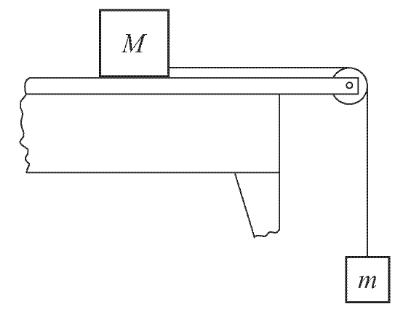
\includegraphics[width=0.45\textwidth]{block2Bodies.png}
\caption{}
\label{block2Bodies}
\end{figure}

\begin{ans}
$a = \frac{mg}{m+M}$; $T = \frac{mMg}{m+M}$.
\end{ans}
\end{ex}

\begin{ex} %Сив79
По наклонной плоскости с углом наклона $\alpha$ скользит тело. Сила трения между телом и плоскостью пропорциональна силе нормального давления тела на плоскость и не зависит от скорости тела. Коэффициент трения между трущимися поверхностями тела и плоскости равен $\mu$. Найти ускорение $a$, с которым скользит тело.
\begin{ans}
$a = g (\sin \alpha - \mu \cos \alpha)$, при $\tg \alpha > \mu$.
\end{ans}
\end{ex}

\begin{figure}[h]
\centering
\begin{subfigure}{.43\textwidth}
  \centering
  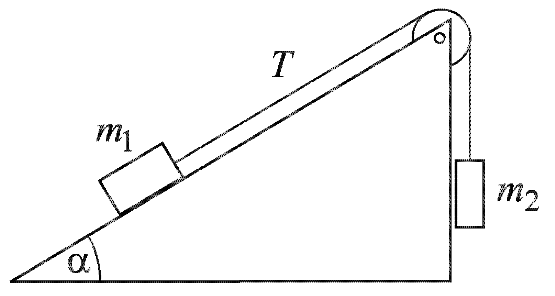
\includegraphics[width=1.0\linewidth]{inclinedPlane.png}
  \caption{}
  \label{inclinedPlane}
\end{subfigure}%
\begin{subfigure}{.57\textwidth}
  \centering
  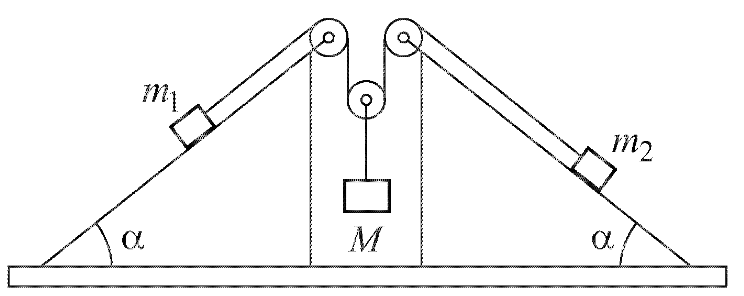
\includegraphics[width=1.0\linewidth]{2InclinedPlanes.png}
  \caption{}
  \label{2InclinedPlanes}
\end{subfigure}
\caption{}
\end{figure}

\begin{ex} %Сив96
На верхнем краю идеально гладкой наклонной плоскости укреплен блок, через который перекинута нить (рис. \ref{inclinedPlane}). На одном ее конце привязан груз с массой $m_1$, лежащий на наклонной плоскости. На другом конце висит груз с массой $m_2$. С каким ускорением $a$ движутся грузы и каково натяжение $Т$ нити? Наклонная плоскость образует с горизонтом угол $\alpha$.
\begin{ans}
$a = \frac{m_1 \sin \alpha - m_2}{m_1 + m_2}g$; $T = \frac{m_1 m_2}{m_1 + m_2}\left( 1+ \sin \alpha \right)g$.
\end{ans}
\end{ex}

\begin{ex} %Сив97
Определить ускорение массы $M$ в системе, изображенной на рис. \ref{2InclinedPlanes}. Массой блоков и силами трения можно пренебречь. Клинья считать закрепленными жестко.
\begin{ans}
$a = \frac{M(m_1 + m_2) - 4 m_1 m_2 \sin \alpha}{M(m_1 + m_2) + 4 m_1 m_2}g$.
\end{ans}
\end{ex}

\qualProblems

\begin{ex}
Надувной матрас заполнен воздухом до давления, превышающего атмосферное. В каком случае давление воздуха в матрасе будет больше: когда человек ляжет на него или когда встанет?
\end{ex}

\begin{ex} %Morin
Два человека тянут веревку в разные стороны, при этом каждый прикладывает силу $F$. Какова сила натяжения веревки?
\begin{ans}
$F$.
\end{ans}
\end{ex}

\begin{ex} %Morin
Два груза равной массы расположены один на другом и помещаются на горизонтальной гладкой поверхности. К нижнему грузу прикладывают горизонтальную силу $F$ и вся система начинает равноускоренно двигаться. Какая сила приводит в движение верхний груз?
\end{ex}

\begin{ex} %Morin
В салоне самолета, который разгонятся на взлетно-посадочной полосе, подвешен в равновесии математический маятник. Будет ли нить этого маятника располагаться вертикально?
\end{ex}

\begin{ex} %Morin
Когда водитель нажимает на педаль газа, автомобиль массы $m$ начинает разгоняться c ускорением $a$, причем $F = ma$, где $F$ - некоторая сила. Что за сила действуют на автомобиль при разгоне?
\end{ex}

\begin{ex} %Morin
Какие санки скатятся быстрее с горки -- с грузом или без груза? Почему?
\end{ex}

\simpleProblems

\begin{ex} %Сив78
На гладкую горизонтальную плоскость помещены три массы $m_1$, $m_2$, $m_3$ связанные нитями между собой и с массой $M$, привязанной к нити, перекинутой через блок (рис. \ref{4Bodies}). 1) Найти ускорение $a$ системы; 2) найти натяжение всех нитей. Трением тел о плоскость и трением в блоке, а также массами блока и нити пренебречь.
\begin{ans}
$a = \frac{Mg}{M + m_1 +m_2 +m_3}$, $T_1 = (m_1 +m_2 +m_3)a$, $T_2 = (m_2 +m_3)a$, $T_3 = m_3 a$.
\end{ans}
\end{ex}

\begin{figure}[h]
\centering
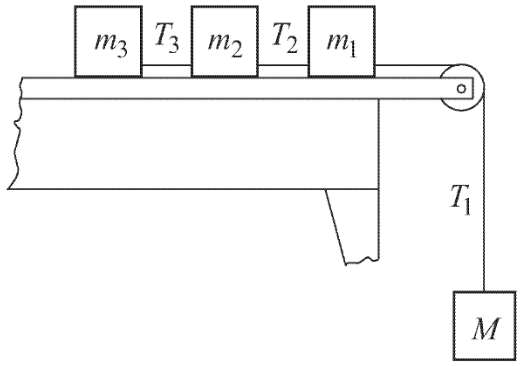
\includegraphics[width=0.5\textwidth]{4Bodies.png}
\caption{}
\label{4Bodies}
\end{figure}

\begin{ex} %Сив80
Два одинаковых тела связаны нитью и лежат на идеально гладком горизонтальном столе, так что нить представляет собой прямую линию. Нить может выдерживать натяжение с силой не более 100 Н. Какую горизонтальную силу $F$ следует приложить к одному из тел, чтобы нить оборвалась?
\begin{ans}
200 H.
\end{ans}
\end{ex}

\begin{ex}
Два бруска массами $m_1$ и $m_2$ расположены один на другом и помещаются на горизонтальной гладкой поверхности. Какую горизонтальную силу $F$ нужно приложить к нижнему грузу массой $m_2$, чтобы выдернуть его из-под верхнего? Коэффициент трения между брусками равен $\mu$.
\end{ex}

\begin{ex} %Сив85-86
Лошадь равномерно тянет сани. Рассмотреть взаимодействие трех тел: лошади, саней и поверхности земли. Начертить векторы сил, действующих на каждое из этих тел в отдельности. Найти величину всех сил, если лошадь и сани движутся с ускорением $a = 20$ см/с\textsuperscript{2}. Масса саней с грузом $M = 0,5$ т, масса лошади $m = 0,35$ т и коэффициент трения саней о снег $\mu = 0,2$.
\begin{ans}
На лошадь со стороны Земли действует сила $F = M(\mu g + a) + ma = 1,17$ кН.
\end{ans}
\end{ex}

\begin{ex} %Сив90
Воздушный шар массы $M$ опускается с постоянной скоростью. Какое количество балласта $m$ надо выбросить, чтобы шар начал подниматься с той же скоростью? Подъемную силу $Р$ шара считать постоянной.
\begin{ans}
$m = 2(M - P/g)$.
\end{ans}
\end{ex}

\begin{figure}[h]
\centering
\begin{subfigure}[t]{.3\textwidth}
  \centering
  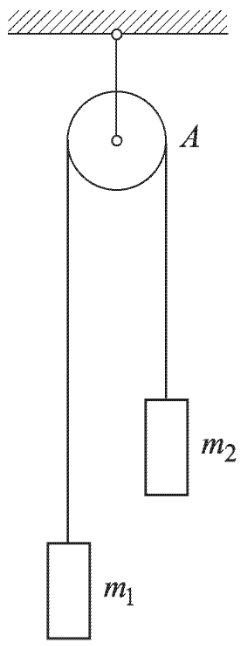
\includegraphics[width=0.7\linewidth]{Atwood.png}
  \caption{}
  \label{Atwood}
\end{subfigure}
\begin{subfigure}[t]{.3\textwidth}
  \centering
  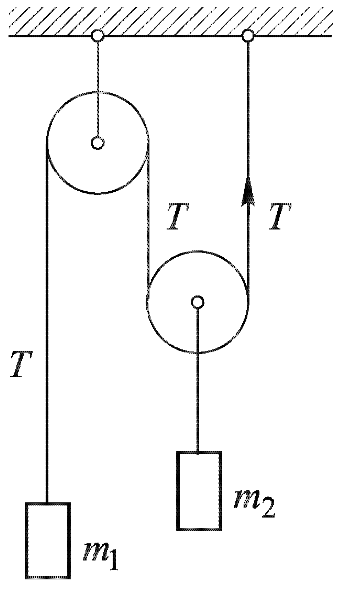
\includegraphics[width=1.0\linewidth]{Atwood2.png}
  \caption{}
  \label{Atwood2}
\end{subfigure}
\begin{subfigure}[t]{.3\textwidth}
  \centering
  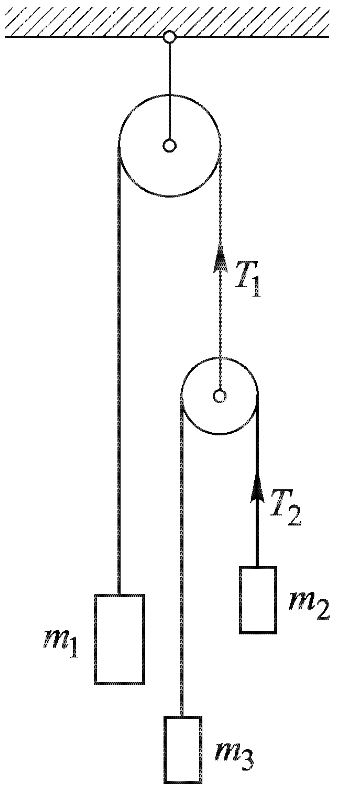
\includegraphics[width=1.0\linewidth]{Atwood3.png}
  \caption{}
  \label{Atwood3}
\end{subfigure}
\caption{}
\end{figure}

\begin{ex}
С вершины наклонной плоскости высотой 5 м и углом наклона к горизонту $45^{\circ}$ начинает соскальзывать тело. Определите скорость тела в конце спуска, если коэффициент трения тела  о плоскость равен 0,19.
\begin{ans}
$ v = \sqrt{2gh(1 - \mu \cot \alpha)} = 9 \textrm{ м/c}.$
\end{ans}
\end{ex}

\begin{ex} %Сив95
Простейшую машину Атвуда, служащую для проверки законов равноускоренного движения, можно схематически представить так: на нити, перекинутой через блок $A$, подвешены две неравные массы, $m_1$
и $m_2$ (рис. \ref{Atwood}). Найти ускорение масс, натяжение нити $T$ и силу $F$, действующую на ось блока этой машины. Блок и нить считать невесомыми, трения в оси блока не учитывать.
\begin{ans}
$a = (m_1 - m_2)g / (m_1 + m_2)$, $T = 2 m_1 m_2 g /(m_1 + m_2)$, $F = 2T$.
\end{ans}
\end{ex}

\begin{ex} %Сив103
Найти ускорения $a_1$ и $a_2$ масс $m_1$ и $m_2$ и натяжение нити $Т$ в системе, изображенной на рис. \ref{Atwood2}. Массой блоков и нитей пренебречь.
\begin{ans}
$a_1 = (2m_1-m_2)g/(2m_1+0,5m_2)$, $a_2 = -a_1/2$, $T=3m_1 m_2g/(4m_1 + m_2)$.
\end{ans}
\end{ex}

\begin{ex}
К концам троса, перекинутого через блок, привязаны бруски с массами $m$ и $M = 4m$, находящегося на гладкой наклонной плоскости с углом наклона $\alpha = 30^{\circ}$ (рис. \ref{inclinedBlock2Bodies}). При каком минимальном значении коэффициента трения между брусками они будут покоиться?
\end{ex}

\begin{figure}[h]
\centering
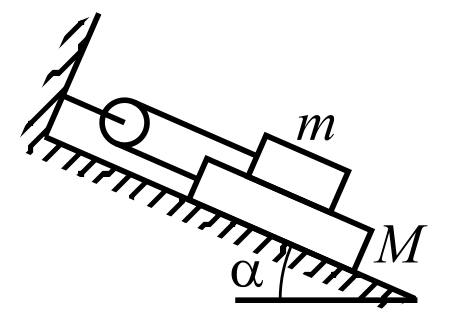
\includegraphics[width=0.3\textwidth]{inclinedBlock2Bodies.png}
\caption{}
\label{inclinedBlock2Bodies}
\end{figure}

\complexProblems

\begin{ex} %Сив104
Найти ускорение массы $m_1$ и натяжения нитей $T_1$ и $T_2$ в системе, изображенной на рис. \ref{Atwood3}. Массой блоков и нитей пренебречь, сил трения не учитывать.
\begin{ans}
$a_1 = \frac{m_1(m_2+m_3)-4m_2m_3}{m_1(m_2+m_3)+4m_2m_3}g$, $T= \frac{8m_1m_2m_3g}{m_1(m_2+m_3)+4m_2m_3}$, $T_2 = T_1/2$.
\end{ans}
\end{ex}

\begin{ex} %Иродов1.65
Небольшое тело пустили вверх по наклонной плоскости, составляющей угол $\alpha  = 15^{\circ}$ с горизонтом. Найти коэффициент трения, если время подъема тела оказалось в $k = 2,0$ раза меньше времени спуска.
\begin{ans}
$\mu = \tg \alpha (k^2-1)/(k^2+1) = 0,16$.
\end{ans}
\end{ex}

\begin{ex} %Сив112
Как будет изменяться скорость тела массы $m$, движущегося вертикально вверх с начальной скоростью $v_0$, если можно считать, что сила сопротивления воздуха пропорциональна скорости тела $F = -rv$, где $r$ -- постоянный коэффициент сопротивления?
\begin{ans}
$v = \frac{mg}{r}\left[ \left( \frac{v_0r}{mg} +1 \right)e^{-\frac{rt}{m}} - 1 \right]$.
\end{ans}
\end{ex}

\clearpage